%%% Research Diary - Entry
\documentclass[11pt,a4paper]{article}

% Working date: The date this entry is describing. Not necessary the date of last edit.
\newcommand{\workingDate}{\textsc{2019 $|$ May $|$ 07}}

% Name and institution must preceed call to researchdiary.sty package
\newcommand{\userName}{Pierre Bréchet}
\newcommand{\institution}{TUM}

% The guts and glory
\usepackage{research_diary}
\usepackage{usrcmd}
\bibliography{bibliography}

% Begin document.
% Use \logoPNG or \logoEPS. If compiling with PDFTeX, use \logoPNG
\begin{document}
% \logoPNG

{\Huge May  7}

\section*{Grad propagation}

The arbitration between spec grad mode and FE grad modes was not finished (cf.
notes of 2019-04-23/24). Tests were then not made on Gaussians but on MNIST. The difficulty of
the model to learn the Gaussian dataset with the new formulation of the
informative regularization might comes from a problem at that level.

Checked out working code on Gaussian that produced thesis plots
(fig/thesis-b/good-good-25gaussian-zt-128-sinkhorn-entropy) to new branch 0405 is under
investigation.

Update: best behaviour for anti-informative dual regularization so far: set the
gradient for the shared networks in both sinkhorn passes, update on the second.
Leave the gradient set for the W network as well (including shared layers)

\paragraph{Latent space} Setting the total latent space dimension to 128 helps the variance collapse effect, as illustrated by '/usr/stud/brechet/computational-ot/fig/merge/master/0506_25gaussian-zt-27/reg-s-no-bn-grad-spec-zt-128/run-rotgan-1/opt.yml'

\paragraph{Simple G} The simplest G network would be a single layer of neurons,
i.e. no hidden units, and ideally only mapping the latent space to x, y values
$x_i = w_{1, 1} g_x + w_{1, 2} g_y + w_{1, i} + b_{1}, y_i = w_{2,1} g_x +
w_{2, 2} g_y + w_{2, i} +  b_{2}$. This is nonetheless not achieved in the
current setup. \\

Update: it might work better with $\beta_1 = 0.5, \beta_2 = 0.95$ in Adam, and larger learning rate.

\paragraph{Comparison with previous working test case} The algorithm run with the same grad behaviour (FE) is not working on the branch master (checked to dev-grad-FE). More precise investigation is to reveal why.

\section*{Sum up}
Tests are in progress for primal anti-informative regularization update, with sinkhorn.
The implementation considers $Q_2$ fixed in the dual udpate, i.e. with gradient mode set to \texttt{'eval'}.

Small $\eps$ are used, with entropic regularizer. Distance is scaled. Both small (27) and big (128) latent space dimensions are tested.

There is always a shift in $U, V$ mean values (they seem to diverge). Good
results were obtained using bias in dual networks, and the absence of bias for
the duals do not prevent the shift from happening\footnote{\url{/usr/stud/brechet/computational-ot/fig/merge/master/toy-25gaussian-mlp/reg-w-primal-sinkhorn/run-rotgan-1/}}

\begin{figure}[!htbp]
   \centering
\begin{subfigure}[t]{0.48\textwidth}
   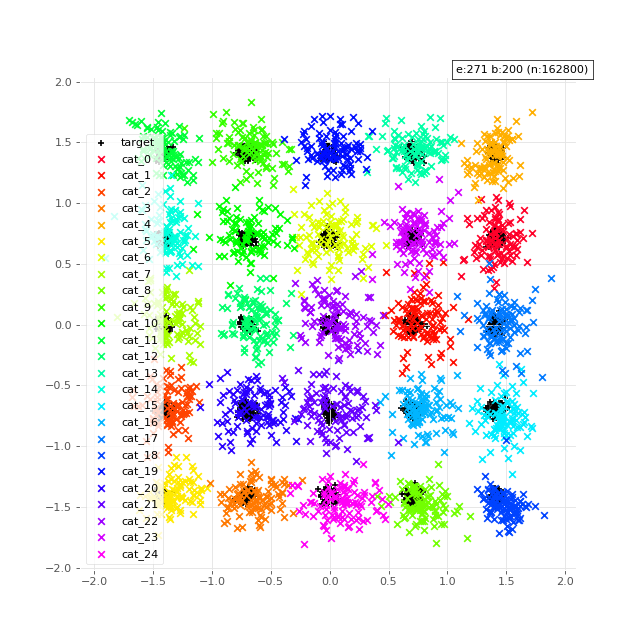
\includegraphics[width=\textwidth,center]{2019-05-07/reg-w-dual/a_zt-128.png}
   \caption{a_zt-128.}
   \label{fig:2019-05-07_reg-w-dual-a}
\end{subfigure}
   \caption{Anti-informative regularization using the dual formulation for the update (previous case). The modes learned are too big.}
   \label{fig:2019-05-07_reg-w-dual}
\end{figure}
\begin{figure}[!htbp]
   \centering
\begin{subfigure}[t]{0.48\textwidth}
   \includegraphics[width=\textwidth,center]{2019-05-07/reg-w-primal/a_zt-27.png}
   \caption{a_zt-27.}
   \label{fig:2019-05-07_reg-w-primal-a}
\end{subfigure}
   \caption{Anti-informative regularization using the primal update (as discussed in the meeting 2019-04-30). The learning is not working yet.}
   \label{fig:2019-05-07_reg-w-primal}
\end{figure}
\begin{figure}[!htbp]
   \centering
\begin{subfigure}[t]{0.48\textwidth}
   \includegraphics[width=\textwidth,center]{2019-05-07/reg-s/a_zt-27.png}
   \caption{Size of latent space: 27}
   \label{fig:2019-05-07_reg-s-a}
\end{subfigure}
   \caption{Informative regularization. Even when using Sinkhorn the modes collapse}
   \label{fig:2019-05-07_reg-s}
\end{figure}
\printbibliography{}
\end{document}
